%\documentclass[12pt, letterpaper]{article}
\documentclass[12pt]{article}
%\usepackage{fontspec}

%\setmainfont{Times New Roman}
%\usepackage{statcourse}
\usepackage{algorithmic}
\usepackage[ruled,vlined]{algorithm2e}
\usepackage{setspace}
\usepackage{times}
\usepackage{verbatim}
\usepackage{epsfig}
\usepackage{amsmath}
\usepackage{amssymb}
\usepackage{array,multirow}
\usepackage{url}
\usepackage{geometry}
\usepackage{threeparttable}
\usepackage{csvsimple}
\usepackage{pgfplots}
\usepackage{pgfplotstable}
\usepackage{tikz}
\usepackage[utf8]{inputenc}
\usepackage{fullpage}
\usepackage{amsmath,amsthm,amsfonts,amssymb,amscd}
\usepackage{lastpage}
\usepackage{enumerate}
\usepackage{fancyhdr}
\usepackage{mathrsfs}
\usepackage{xcolor}
\usepackage{listings}
\usepackage{hyperref}
\graphicspath{ {./images/} }
\usepackage{appendix}
\usepackage[final]{pdfpages}
\usepackage{pdflscape}
\usepackage{xcolor}
\usepackage{listings}
\usepackage{color}
%\usepackage{subfigure}
\usepackage{subfig}
\usepackage{graphicx}
\renewcommand{\baselinestretch}{.88}
\geometry{letterpaper,left=2.54cm,right=2.54cm,top=2.54cm,bottom=2.54cm}



% Include other packages here, before hyperref.

% If you comment hyperref and then uncomment it, you should delete
% egpaper.aux before re-running latex.  (Or just hit 'q' on the first latex
% run, let it finish, and you should be clear).
\usepackage{cleveref}


%\statcoursefinalcopy
%\linespread{1.0}

\begin{document}
	
	\noindent\textbf{1. Introduction}
	
	Yelp, a platform for customers to write reviews and ratings of the businesses, published a subset of their data set, containing four JSON files about the reviews and the information of businesses and users. In this report, we intend to provide useful, actionable suggestions to business owners in order to improve their ratings based on the information contained in reviews, and the attributes of the businesses. Owing to the enormous differences among different categories of businesses, we mainly provide suggestions to "burger businesses" in this report. After preprocessing the data sets, we have 65154 user reviews for 1428 burger businesses in total, giving an average of 46 reviews for a burger business. We are mainly interested in the finding following two relationships: (1) the review scores (on a 1-5 scale) as summarized in the left figure of \cref{Figure:hist} and the review texts; and (2) the overall scores for businesses as summarized in the right figure of \cref{Figure:hist} and the attributes of the businesses. Based on findings from these two aspects, we are able to provide in-depth suggestions to burger business owners.
	
	\begin{figure}[h!]
		\centering
		\begin{subfigure}
			\centering
			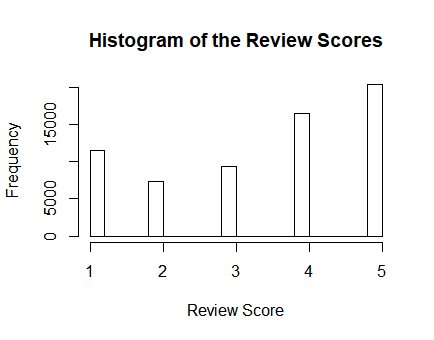
\includegraphics[scale=0.6]{Review_Summary.png}
		\end{subfigure}%
		\begin{subfigure}
			\centering
			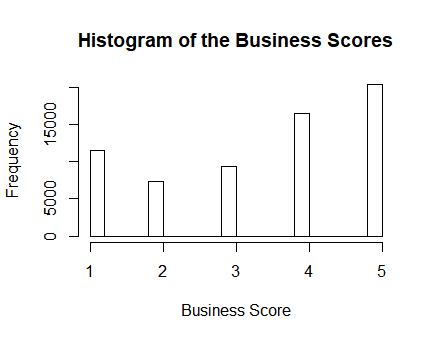
\includegraphics[scale=0.6]{Business_Summary.png}
		\end{subfigure}%
		\caption{Histograms for Review Scores and Business Scores}
		\label{Figure:hist}
	\end{figure}
	
	%The rest of the report is organized as follows. We introduce the details of data analysis, including preprocessing and model building of the data, in Section 2. We provide overall analytical insights and a data-driven action plan based on the aforementioned data analysis in Section 3. We state the strengths and weaknesses of the model in Section 4, and our contributions in \textbf{Contributions}.
	
	\noindent\textbf{2. Statistical Analysis}
	
	In this section, we provide detailed narratives of the process of data analysis. We first clean and extract useful information for the text data in 2.1, and then use lasso to reduce the high dimension of the text data in 2.3, and use regression to fit the proper model in 2.4.
	
	\noindent\textbf{2.1 Data Cleaning}
	
	In order to extract useful information from the reviews, we need to pre-process the text data. We were interested in those burger shops whose "categories" contains "burger", for the restaurants of burger, the evaluation models are built from two sources of information: (a) The 65154 reviews of 1428 restaurants. (b) The restaurant attributes provided by yelp. For (b), we grep through the attributes and finally got 15 categorical variables like \textit{RestaurantsDelivery}, \textit{HasTV}, etc.
	For (a), the analysis of restaurants reviews could be described as follows:
	
	(1) Merge "review.json" and "business.json" by "business\_id" in order to reflect the information of reviews on the properties of their corresponding businesses.
	(2) Select one "burger" restaurants' reviews and remove duplicates lines. After which the total reviews is reduced to 65154.
	(3) Remove all the punctuation and changed all words to lower case.
	(4) We noticed that there exist typos and non-English words, so we removed them and left only the English words.
	(5) Tokenize negative words, such as "no", "not", "not\_much" into the adjacent words to convey the real feelings of the reviewers, such as converting "not clean" to a single word "no\_clean";
	(6) Break the strings into lists of words and remove stop words. Notice that those "no", "not" won't be mistakenly removed since we have already combined them with their nearest words.
	(7) Lemmatize. That is, Convert singular and plural nouns into singular. Unify verbs in different tenses into the general present tense.
	(8) Count the frequency of each word and remove all the words occurring only once or twice, since they are mostly typos or nonsense.
	
	\noindent\textbf{2.2 TF-IDF (Term Frequency-Inverse Document Frequency)}
	
	We first obtain a sparse matrix based on the frequencies of the occurrences of a word for each text review, where rows for the text reviews and columns for words that occur three or more times in all reviews. We have 65313 reviews in total for all "burger" restaurants, and 21848 words that occur more than twice, resulting a sparse matrix of 65313*21848 dimension. In this case, however, if a word occurs more often than others in general, it is more likely to occur more frequently in a review, such as "burger" in our case, which is unfair to other words. Therefore, we use TF-IDF (Term Frequency-Inverse Document Frequency) to offset these effects. TF-IDF can be mathematically characterized by
	\begin{equation}
	TFIDF(\omega,t) = TF(\omega,t)\times IDF(\omega,t) = \frac{\mathrm{\#\omega~in~t}}{\mathrm{\#words~in~t}}\times log(\frac{\mathrm{\#words~in~t}}{\mathrm{\#reviews~that~contains~\omega}})
	\end{equation}
	where $\omega$ is a word and $t$ represents a review. But in essence, Idf is a weighting that tries to suppress noise, and simply believes that words with lower text frequency are more important, and words with higher text frequency are more useless. Obviously, this is not completely correct especially when some certain words/typos may be evaluated as important words. It is not reasonable to simply take words with top Tf-Idf scores.
	
	\noindent\textbf{2.3 Lasso}
	
	After transforming reviews to document-term-matrix, we have a scaled sparse 65313*21848 matrix. Although $n>p$ which cannot be considered as high-dimensional regime, we still need to reduce the dimension of the variables (i.e., words). We adapt lasso to shrink non-significant coefficients to zero and then define the selection set $\hat{S}$ as follows:
	\begin{equation}
	\begin{aligned}
	\hat{\beta}^\lambda &= argmin_{\beta \in \mathbb{R}^p} ||y-X\beta||_2^2+\lambda||\beta||_1\\
	\hat{S}^\lambda &= \{k:\hat{\beta}_k^\lambda \neq 0\}
	\end{aligned}
	\end{equation}
	where $X \in\mathbb{R} ^{n*p} $ is the design matrix, $y \in \mathbb{R}^n$ is a vector of outputs, and $\lambda$ is a regularization parameter that controls the size of the selection set.
	
	There are several existing methods for model selection, such as cross-validation, AIC/BIC scores, hypothesis testing, knockoffs, and stability methods. In our context, we use \textit{stability selection}\cite{meinshausen2010stability}, whose goal is to provide an improvement on existing basic methods (i.e. Lasso in our project) while controlling the number of false discoveries. The algorithm helps to reduce the sensitivity to the choice of regularization parameters by subsampling on the observations. Based on Lasso, we use the algorithm seven times using seven equally spaced thresholds (i.e., $\pi_{thr}\in \{0.6, 0.65, 0.7, 0.75, 0.8, 0.85, 0.9\}$), take the intersect of the return variable set $\hat{S}^{stable}$, resulting in selecting 765 words out of 21848. The results vary little when setting $\pi_{thr}\in (0.6, 0.9)$ and we take intersection for robustness.
	
	\begin{comment}
	\begin{algorithm}
	\caption{Stability Selection Algorithm}
	\label{algorithm}
	\begin{algorithmic}[1]
	\REQUIRE data set $Z_1, \dots, Z_n$.
	\STATE Define a candidate set of regularization parameters $\Lambda$ and a subsample number N (=100).
	\STATE For each value of $\lambda \in \Lambda$, do:\\
	(a) Start with the full dataset $Z_{full} = Z_1, \dots, Z_n$\\
	(b) For each i in $1, \dots,N$, do:\\
	i. Subsample from $Z_{full}$ without replacement to generate a smaller dataset of
	size $\lfloor n/2 \rfloor$, given by $Z_{i}$.\\
	ii. Run the selection algorithm on dataset $Z_{i}$ with parameter $\lambda$ to obtain a
	selection set $\hat{S}_{(i)}^\lambda$.\\
	(c) Given the selection sets from each subsample, calculate the empirical selection
	probability for each model component:
	$\hat{\Pi}_k^\lambda=P(k \in \hat{S}^\lambda)=\frac{\sum_{i=1}^{N} I(k \in \hat{S}_{(i)}^\lambda)}{N}$
	The selection probability for component k is its probability of being selected by
	the algorithm.
	\STATE Given the selection probabilities for each component and for each value of $\lambda$, construct
	the stable set according to the following definition:\\
	$\hat{S}^{stable} = \{k:\max_{\lambda \in \Lambda }\hat{\Pi}_k^\lambda \geq \pi_{thr}\}$\\
	where $\pi_{thr}$ is a predefined threshold varied from 0.6 to 0.9.
	\RETURN $\hat{S}^{stable}$
	\end{algorithmic}
	\end{algorithm}
	\end{comment}
	
	
	\noindent\textbf{2.4 Multiple T-test for reviews}
	
	After stability selection, we conducted multiple-testing for the 765 words, with the Bonferroni correction, 253 words with $p = 0.05/765 =6.54*10^-5$ are considered significant to the overall rating scores. The results of the top five variables based on p-value is summarized in \cref{tab:regress}.
	
	\begin{table}[htp]
		\centering
		\caption{T-test Summary (Top 10 variables)}
		\label{tab:regress}
		\resizebox{0.8\textwidth}{!}{
			\begin{tabular}{ccccccccccc}
				\hline\hline
				words&occurence&pval&tscore\\
				great&29060&0&47.4054425559631\\
				best&10642&2.75845242066736e-243&33.4542380847868\\
				worst&2238&2.90066315434987e-215&-31.4349060901696\\
				amazing&6170&3.22304171253052e-190&29.5173425939315\\
				delicious&9390&9.48495435969436e-166&27.5191839459281\\
				\hline
		\end{tabular}}
		\label{tab:1}
	\end{table}
	
	As we can see, words like "great", "best" really have an impact on the rating, however, such words can't provide any valid information for suggestions. To find out the suggested information hidden in the words, We manually selected dozens of the last 253 words and categorized these indicator words into 4 dimensions. \textbf{FOOD}\{ cold,awful,mediocre, etc\}, \textbf{ENVIRONMENT}\{dirty,filthy,stale, etc\}, \textbf{SERVICE}\{rude, unfriendly, unprofessional, etc\} and \textbf{ETHNICITY}\{racist\}. For each restaurant, we looked through all indicator words in the four dimensions, and highlight the word if over $1\%$ reviews mentioned this word. After that, the suggestions are provided through the specific highlighted words.
	
	For example, if the word \textit{cold} in \textbf{FOOD} dimension is highlighted, then the suggestion from this dimension would contain \{\textbf{Improve hygiene and speed of cooking.}\} for better food services.
	
	\noindent\textbf{2.5 Regression tree on attributes}
	
	Based on attributes of every shop, we build up a regression tree to help to see how those facilities and services affect the rating. All the attributes include: RestaurantsDelivery, RestaurantsTakeOut, BusinessAcceptCreditCards, RestaurantsReservations, HasTV, RestaurantsGoodForGroups, RestaurantsPriceRange, NoiseLevel, Alcohol, OutdoorSeating, RestaurantsAttire, WiFi, GoodForKids, BikeParking. Since all of them are categorical variables, we decided to use a tree structure, which is also convenient for visualization, to help the business owners to find out what is customers’ preference. We use all the 65154 observations to build up the tree since the numbers of reviews from different should be considered as weights. In our project, we consider the stars as a quantitative variable so the method of building up the tree is “anova”. The tree built up by the package \textit{rpart}:\\
	\begin{figure}[h!]
		\centering
		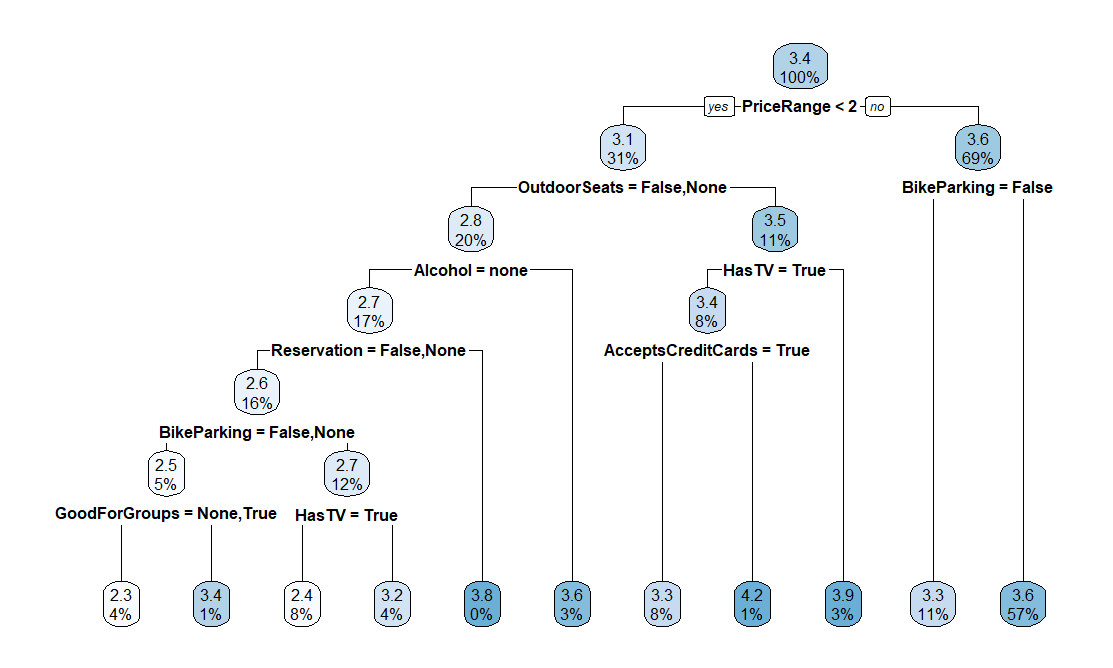
\includegraphics[width=15cm]{RegTree.png}
		\caption{Regression Tree based on attributes}
		\label{fig:ins}
	\end{figure}
	
	As we do further t-test on these ten variables, we selected the top 5 and give advice mainly on these five variables with the highest importance: Price range (3219.1), Outdoor Seating (1500.2), Whether has TV (1344.9), Alcohol (1342.6) and Bike Parking (754.6).
	
	\noindent\textbf{3. Insights \& Action Plan}
	
	As a result of the aforementioned statistical analysis, we obtain some insights into the businesses based on the review texts and the attributes of the businesses. We provide suggestions to burger business owners in the following nine aspects: \textbf{Service, Food, Environment, and Ethnicity}, from reviews; and \textbf{Price Range, Outdoor Seating, TV, Alcohol, Bike Parking}, from attributes, all of which are found to be highly related to review scores. For example, for Meatheads at 1305 S Neil St, IL, a typical suggestion is summarized in \cref{fig:ins}. Besides the suggestions, we also provided the average rating of that restaurant, the percentile of its rating among all restaurants, the distribution of the rating. A cloud plot for the significant words in each restaurant's reviews will also be drawn in the \href{https://jiawei98.shinyapps.io/UI_module3/}{\textbf{\textcolor{blue}{ShinyApp}}}.
	
	\begin{figure}[htbp]
		\centering
		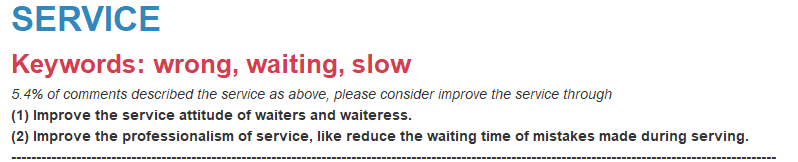
\includegraphics[width=15cm]{typical.png}
		\caption{A typical suggestion at 1305 S Neil St, IL}
		\label{fig:ins}
	\end{figure}
	
	\noindent\textbf{4. Strengths and Weaknesses}
	
	\noindent\textbf{4.1 Strengths}
	
	1. We selected our indicators from various sources (review, attributes) and using various methods (lasso, t-test, and regression tree), which guarantees the significance and accuracy of our model.
	
	2. We give separate suggestions to the individual physical store of the chain stores, since we believe they may perform differently. For example, we give suggestions on providing outdoor seats to the McDonald's at 3051 E Washington Ave, Madison, but not to McDonald's at 4020 Milwaukee St, Madison.
	
	3. The method is applicable and improvable. We can apply it to larger data sets or data set for other industries.
	
	4. Stability selection (based on lasso) improve the performance of penalized regression. By subsampling, it could control the number of falsely discovered variables lower than a pre-defined threshold. Also, it avoids the sensitivity to the regularization parameter,
	
	
	\noindent\textbf{4.2 Weaknesses}
	
	1. Due to the size of our data set, the helpful decision can't be useful for all restaurants. For those burger restaurants with 1ess than 20 reviews, the suggestions are usually extracted from less than 5 reviews and suffers from great uncertainty.
	
	2. Only through separating the sentience, combining some specific words, removing stop words and lemmatizing, some complex hidden information in the sentences is difficult to reveal. To refine the central idea of the review, we might need some deep learning methods. However, this is another big topic.
	
	3. Especially during this pandemic of Covid-19, our advice might be less effective affected by special policies. For example, it is very important for restaurants to provide take-out now and the importance of this aspect (given by regression tree) would increase to a much higher level. Because of the limitation of the data set, all the advice are only for reference under regular circumstances.
	
	\pagebreak
	\section*{Contributions}
	
	\noindent JH: Section 2.1, 2.4, 4 of the Summary. Slides 13-18. Code for data cleaning and shiny app. \\
	YQ: Section 2.2, 2.3, 2.5 of the Summary. Slides 5-12. Code for main model building.\\
	SZ: Section 1,3 of the Summary. Slides 1-4, 19-22. Code for rendering plots and tables.\\
	
	\bibliographystyle{plain}
	\bibliography{reference.bib}
	
	
	
	
\end{document}

